\documentclass[manuscript,screen,review]{acmart}
\usepackage{graphicx}
\usepackage{tabularx}
\usepackage{array}
\usepackage{booktabs}
\usepackage{ragged2e}
\usepackage{enumitem}
\newcolumntype{L}{>{\RaggedRight\arraybackslash}X}
\newcolumntype{P}[1]{>{\RaggedRight\arraybackslash}p{#1}}
\newcommand{\tblhead}[1]{\textbf{#1}}
\setcopyright{none}
\settopmatter{printacmref=false}
\acmJournal{JACM}
\acmYear{2026}
\acmSubmissionID{}
\renewcommand\footnotetextcopyrightpermission[1]{}
\begin{document}
\title{External IoT Retrofit for Remote Monitoring and Control of a Rheem EW1-50RP Water Heater}
\author{José Paca}
\affiliation{\institution{Universidad de Ingeniería y Tecnología (UTEC)}\city{Lima}\country{Peru}}
\author{Daniel Casquino}
\affiliation{\institution{Universidad de Ingeniería y Tecnología (UTEC)}\city{Lima}\country{Peru}}
\author{Nicolas Stigler}
\affiliation{\institution{Universidad de Ingeniería y Tecnología (UTEC)}\city{Lima}\country{Peru}}
\author{Sofia Ku}
\affiliation{\institution{Universidad de Ingeniería y Tecnología (UTEC)}\city{Lima}\country{Peru}}
\begin{abstract}
This paper presents an Internet of Things (IoT) system for remote monitoring and external control of a Rheem EW1-50RP
electric storage water heater without modifying its internal electronics or mains supply.
The system integrates an ESP32-WROOM microcontroller, an ESP32-CAM module for optical temperature acquisition,
a TCS34725 RGB sensor for monitoring the heating indicator, and a Hall-effect pulse input for a separate flow-measurement channel.
Temperature readings are extracted from images of the heater's original display using an optical character recognition (OCR)
pipeline with Sharp preprocessing and configurable seven-segment or Tesseract.js recognition. The ESP32 processes sensor readings, controls low-voltage servomotors, and exchanges
commands and telemetry through Wi-Fi and MQTT. A Node.js service integrates MQTT communication, image processing, and
WebSocket messaging with a web-based dashboard for remote monitoring and control. Mounted optical calibration yielded distinct red, green, and unlit pilot responses, and a tape-mounted power servo registered a button press at a configured angle of 29 degrees. The implementation combines these observations with guarded commands and separates the displayed water temperature from the selected temperature setpoint.

\end{abstract}
\keywords{Internet of Things, water heater, ESP32, remote monitoring, optical character recognition, MQTT}
\maketitle
\section{Introduction}
Domestic electric storage water heaters may require users to be physically near the appliance to monitor its temperature and
operate its controls. 
The Rheem EW1-50RP (50 L, 1500 W) is the reference appliance for this project.
It measures and displays the temperature at the center of its tank, controls heating through an internal thermostat,
and provides an AI Smart operating mode~\cite{rheemmanual}.
However, access to its temperature readings and control interface is restricted to the appliance's physical panel.

This project addresses this limitation through an external Internet of Things (IoT) system that integrates sensing,
mechanical actuation, and wireless communication without modifying the heater's internal electrical circuitry.
An ESP32-CAM captures images of the original temperature display for optical recognition, while an RGB sensor monitors the heating indicator.
Additionally, a Hall-effect sensor supplies a separate pulse-acquisition channel for flow and accumulated-volume calculations.

An ESP32-WROOM microcontroller coordinates sensor acquisition, servo actuation, and communication through the MQTT protocol.
A Node.js application service processes camera images, manages MQTT messages, and communicates with a web-based dashboard
through WebSocket. This architecture enables remote visualization of temperature readings, sensor measurements, and device information,
while allowing control commands to be transmitted to the embedded controller.

The system is designed around the Rheem EW1-50RP while preserving the heater's original temperature regulation and
electrical protection mechanisms.
Its modular architecture also provides a reference for extending monitoring and external control capabilities to other
appliances with local-only interfaces.


\section{Problem Statement}
\Needspace{6\baselineskip}
\subsection{Problem Description and Justification}
For the selected Rheem heater, the user must approach the panel to read the tank-center temperature or operate its buttons~\cite{rheemmanual}. This limits remote preparation of hot water and makes the distinction between heating, heat preservation, standby, and power-off difficult to observe from another room. The practical problem is to recover panel information and operate the existing controls through an external retrofit while preserving the appliance's internal regulation and electrical protections.

A useful monitoring interface must distinguish the water-temperature readout from the selected setpoint and treat unreadable observations explicitly. Flow information provides a complementary measurement of water passing through a sensor~\cite{lee2021}; it is different from heating time or electrical energy. The prototype therefore combines optical panel observations, mechanical button actuation, and a separate flow-acquisition channel in a local wireless application.

\section{Theoretical Framework}
\Needspace{6\baselineskip}
\subsection{Panel Readout and Heater Operation}
The EW1-50RP displays the water temperature measured near the center of the tank. Its panel includes power and temperature-adjustment buttons and a heating indicator; the manual associates red with heating and green with heat preservation~\cite{rheemmanual}. When the user changes the setpoint, the selected number flashes before the panel returns to the current-temperature readout. These two quantities require separate variables in the monitoring system.

A camera facing the display can acquire digits without accessing the internal electronics. Tongbai describes an ESP32-CAM instrument-readout system with server-side image recognition~\cite{tongbai2024}. The present system adopts that acquisition principle. An independent TCS34725 measures red, green, blue, and broadband clear-channel light through an I\textsuperscript{2}C interface~\cite{adafruitcolor}. An opaque sleeve limits the pilot measurement to the same optical field during calibration and use.

\Needspace{6\baselineskip}
\subsection{Flow Pulses and External Actuation}
A Hall-effect turbine sensor produces pulses as water moves its rotor. Volume follows the counted pulses divided by a pulses-per-liter factor, and flow rate also depends on the duration of the counting interval. The factor is a calibration parameter for the actual sensor and operating conditions. The prototype's firmware uses 450 pulses/L as its configured value for the separate channel.

Three servo positions are assigned to power, increase, and decrease. Each mechanism has its own rest and press angles. Commercial button pushers illustrate the external mechanical approach~\cite{switchbot}. Because a power button can either wake the panel or change its state, a reliable routine distinguishes an initial wake press from the requested action.

\Needspace{6\baselineskip}
\subsection{Communication and Preprocessing}
The ESP32 controller counts pulses and samples the RGB sensor. A separate ESP32-CAM provides JPEG images over HTTP, and the Node.js service recognizes the display outside the embedded control loop. Wi-Fi carries HTTP and MQTT traffic; WebSocket connects the service to the dashboard. Validated commands reach the controller through MQTT, while missing, stale, or ambiguous measurements remain unavailable rather than becoming numerical zero.

\section{State of the Art}
Eight studies provide the scientific foundation for the system's design.
Each addresses a specific aspect of water monitoring, water-heater control,
optical data acquisition, or user interaction.
Together, these studies inform the architectural decisions adopted in this work.

\Needspace{6\baselineskip}
\subsection*{A1. Smart monitoring of water use}
Palermo et al.~\cite{palermo2022} review smart technologies for water resource management,
particularly at building scale. Their overview connects sensing and communication with
information about occupants' water use. This supports the integration of a monitoring
interface that presents observations from the prototype. Providing such information,
however, does not establish water or energy savings for the appliance considered here.

\Needspace{6\baselineskip}
\subsection*{A2. Control of domestic water heating}
Ritchie et al.~\cite{ritchie2022} investigate centrally coordinated control schedules for
multiple electric water heaters. Their simulations compare hot-water delivery strategies
and constrained peak loads. The study motivates distinguishing control actions from
measured outcomes. Unlike their coordinated scheduling approach, the system developed
here interacts with one heater through its existing physical interface, preserving the
original electrical control mechanisms.

\Needspace{6\baselineskip}
\subsection*{A3. Networked water-consumption monitoring}
Slan\'{y} et al.~\cite{slany2020} develop a modular smart-metering platform using
LoRaWAN and evaluate it in laboratory and residential conditions, including leakage detection.
Their work demonstrates the relevance of transmitting water-use measurements for monitoring.
The present system instead uses a Hall-effect turbine flow sensor and Wi-Fi communication.


\Needspace{6\baselineskip}
\subsection*{A4. Flow measurements outside the pipe}
Riboldi et al.~\cite{riboldi2023} investigate contactless monitoring with ultrasonic
transducers and external electrodes clamped onto plastic pipes. Their hydraulic-loop
experiments show an alternative to inserting sensors into the fluid path. This distinguishes
non-invasive access to the heater electronics from non-invasive flow measurement:
our turbine sensor still requires water to pass through its body. Their results do not
validate our sensor or its installation.

\Needspace{6\baselineskip}
\subsection*{A5. Demand and flow data}
Lee and Yim~\cite{lee2021} analyze domestic hot-water energy and flow demand using smart-meter data.
This supports measuring use rather than treating powered time as water consumption.


\Needspace{6\baselineskip}
\subsection*{A6. Optical reading of a display}
Tongbai~\cite{tongbai2024} uses an ESP32-CAM to capture a digital instrument display
without a communication port and recognizes its seven-segment digits on a web server.
We apply the same capture-and-recognize approach to the Rheem visor, subject to testing
its geometry and lighting. Recognition accuracy reported for the calibration instrument
cannot be transferred to the heater display without corresponding tests.

\Needspace{6\baselineskip}
\subsection*{A7. Advanced scheduling as a boundary}
Shen et al.~\cite{shen2021} study data-driven electric water-heater scheduling using
robust model predictive control. Their evaluation combines a real-world dataset with
simulations of a central water heater. Their work explains why demand information may
be useful later.

\Needspace{6\baselineskip}
\subsection*{A8. User-centered smart-home services}
Chang and Nam~\cite{chang2021} examine smart-home service preferences and adoption
through a survey of potential users in South Korea. Their findings associate service
preferences with adoption intentions and identify interest in safety and convenience.
This motivates presenting clear status information and accessible controls. It does not
constitute a usability evaluation of our interface or demonstrate energy savings.

\Needspace{6\baselineskip}
\subsection{Proposed Contribution}
These sources separately address hot-water control, flow data, optical readout, and user interaction.
Our contribution is to combine optical observations of the specific EW1-50RP with removable
button actuation while retaining the heater's original controls, and to demonstrate flow
acquisition separately. The integration addresses monitoring and external interaction;
its evaluation must distinguish observed device states, recognition results, and control
requests rather than infer energy savings from connectivity alone.

\section{Objectives}
\Needspace{6\baselineskip}
\subsection*{General Objective}
Develop and evaluate a removable external IoT prototype for monitoring the panel and controlling the existing buttons of a Rheem EW1-50RP water heater, while leaving its internal controller and mains connection untouched.

\Needspace{6\baselineskip}
\subsection*{Specific Objectives}
\begin{enumerate}[label=SO\arabic*.]
\item Read the heater's original temperature display with a camera and classify the pilot using shielded RGB measurements.
\item Acquire Hall-effect sensor pulses in a separate flow channel and calculate flow rate and accumulated volume from the configured pulse factor.
\item Present the sensor information and controller state in a wireless dashboard, including unavailable readings.
\item Coordinate external power, increase, and decrease button mechanisms with validated commands and explicit press-and-return positions.
\item Compare the optical calibration, recorded button response, and implemented control logic with their corresponding observations and software checks.
\end{enumerate}

\Needspace{6\baselineskip}
\subsection*{Scope}
The prototype targets one EW1-50RP and reads the temperature reported by its original sensor and display. The camera and RGB sensor observe the front panel, while low-voltage servos operate the existing buttons. The Hall-effect channel is evaluated separately from the heater plumbing. The dashboard distinguishes the current temperature, selected setpoint, pilot observation, and communication availability. The heater's own thermostat remains responsible for thermal regulation.

\section{Methodology}
\Needspace{6\baselineskip}
\subsection{Reference Appliance and System Components}

The system was developed for the Rheem EW1-50RP electric storage water heater, which has a nominal capacity of 50 L
and an electrical power rating of 1500 W at 220--240 V. The appliance includes an internal temperature controller,
a digital display, and physical buttons for operating the heating system~\cite{rheemmanual}.

The proposed IoT architecture extends the appliance's monitoring and control capabilities through external sensing,
mechanical actuation, and wireless communication. An ESP32-WROOM microcontroller serves as the central embedded
controller, while an ESP32-CAM operates as an independent image acquisition node.

Table~\ref{tab:components} summarizes the components and their corresponding roles within the system.

\begin{table*}[htbp]
\centering
\caption{Main hardware and software components of the IoT system.}
\label{tab:components}
\small
\renewcommand{\arraystretch}{1.12}
\begin{tabularx}{\textwidth}{@{}P{2.7cm} P{2.8cm} L@{}}
\toprule
\tblhead{Function} & \tblhead{Component} & \tblhead{Description} \\
\midrule

Central controller
& ESP32-WROOM-32
& Coordinates sensor acquisition, servo actuation, and MQTT communication over Wi-Fi. \\

Display capture
& ESP32-CAM / OV2640
& Serves JPEG images of the original display over HTTP. \\

Pilot sensing
& TCS34725 RGB sensor
& Acquires raw RGBC readings from the pilot through I\textsuperscript{2}C. \\

Flow acquisition
& SEA ZJ-S201 Hall-effect flow sensor
& Provides the pulse-count input of the separate flow channel; a configured factor converts counts into flow rate and accumulated volume. \\

Mechanical actuation
& Low-voltage servomotors
& Press and release the original panel buttons. \\

Wireless communication
& Wi-Fi and MQTT
& Enable the exchange of control commands and telemetry between the ESP32 and application infrastructure. \\

Image processing
& Sharp, seven-segment reader, Tesseract.js
& Preprocess images and provide configurable numerical readers for the original display. \\

Application service
& Node.js and WebSocket
& Manage image processing, MQTT messaging, application state, and bidirectional communication with the web interface. \\

User interface
& Web-based dashboard
& Presents device information and sensor measurements and provides controls for transmitting commands to the system. \\

\bottomrule
\end{tabularx}
\end{table*}

\Needspace{6\baselineskip}
\subsection{System Architecture}

The system follows a distributed architecture composed of an embedded control subsystem, an image acquisition subsystem,
a communication layer, and a web-based application.
Figure~\ref{fig:architecture} illustrates the principal components and the communication paths between them.

\begin{figure*}[!t]
    \centering
    \resizebox{0.96\linewidth}{!}{\resizebox{\textwidth}{!}{%
\begin{tikzpicture}[
  font=\small,
  box/.style={draw, rounded corners, align=center, text width=3.4cm, minimum height=1.15cm, inner sep=6pt},
  link/.style={-{Latex[length=2mm]}, thick},
  labeltext/.style={font=\footnotesize, align=center, fill=white, inner sep=2pt}
]
\node[box, text width=4cm] (heater) at (0,0) {Water heater panel\\Numeric display and pilot\\Power / increase / decrease};
\node[box] (camera) at (-4,-2.5) {ESP32-CAM\\Display image capture};
\node[box] (rgb) at (0,-2.5) {RGB sensor\\Pilot light acquisition};
\node[box] (servos) at (4,-2.5) {Three servos\\Power / increase / decrease};
\node[box] (backend) at (-4,-5.4) {Application backend\\Image preprocessing / OCR\\MQTT client};
\node[box, text width=1.15cm, inner sep=4pt] (broker) at (-1,-5.4) {MQTT\\broker};
\node[box] (controller) at (2,-5.4) {ESP32 controller\\RGB input / flow pulse ISR\\Queued actuator control};
\node[box] (dashboard) at (-4,-8) {Dashboard\\Measurements and requests};
\node[box, dashed] (flow) at (2,-8) {Separate flow channel\\Hall-effect pulse sensor};

\draw[link] (heater.west) -| node[labeltext, pos=0.75, left] {Display\\image} (camera.north);
\draw[link] (heater.south) -- node[labeltext, right] {Pilot light} (rgb.north);
\draw[link] (servos.north) |- node[labeltext, pos=0.3, right] {Mechanical\\button press} (heater.east);
\draw[link] (camera.south) -- node[labeltext, right] {Wi-Fi / HTTP\\JPEG capture} (backend.north);
\draw[link] (rgb.south) -- node[labeltext, right] {I\textsuperscript{2}C} (controller.north);
\draw[link] (controller.east) -| node[labeltext, pos=0.75, right] {PWM} (servos.south);
\node[labeltext] at (-1,-4.3) {Wi-Fi / MQTT\\Telemetry and commands};
\draw[thick, {Latex[length=2mm]}-{Latex[length=2mm]}] (backend.east) -- (broker.west);
\draw[thick, {Latex[length=2mm]}-{Latex[length=2mm]}] (broker.east) -- (controller.west);
\draw[thick, {Latex[length=2mm]}-{Latex[length=2mm]}] (backend.south) -- node[labeltext, right] {WebSocket} (dashboard.north);
\draw[link, dashed] (flow.north) -- node[labeltext, right] {Pulse input / ISR} (controller.south);
\end{tikzpicture}%
}
}
    \caption{Prototype architecture. The camera-to-server recognition path adapts the optical acquisition principle of Tongbai~\cite{tongbai2024}; the control, pilot, and separate flow paths are the implementation developed here.}
    \label{fig:architecture}
\end{figure*}

The ESP32-WROOM operates as the central embedded controller and interfaces with the sensors and servomotors.
The TCS34725 communicates through the I\textsuperscript{2}C protocol, while the flow sensor provides digital
pulses that are counted through a GPIO interrupt.
These measurements are processed periodically to obtain sensor readings and water consumption metrics.

The ESP32-CAM operates as an independent Wi-Fi node.
Instead of transmitting camera data directly to the ESP32 controller, it exposes an HTTP endpoint through which
the application service retrieves images of the heater's display.
This separation allows image processing to be performed outside the embedded control loop.

The communication layer uses an MQTT broker to exchange messages between the ESP32 and the application service.
The embedded controller subscribes to command topics and publishes telemetry and device state messages.
The application service receives these messages and communicates with the web interface through WebSocket.

User interactions generate WebSocket messages that are processed by the application service and translated into MQTT commands.
These commands are received by the ESP32, which executes the corresponding control routines.

\Needspace{6\baselineskip}
\subsection{Temperature Acquisition and Processing}

Temperature information is acquired from the heater's original digital display using the ESP32-CAM.
The camera provides JPEG images through its HTTP interface, which are requested and processed by the Node.js application service.

The image processing pipeline uses Sharp to perform operations such as cropping, resizing, grayscale conversion, and intensity adjustments.
The selected operations align and isolate the digits before recognition.

The application selects either a geometric seven-segment reader or Tesseract.js to identify the numerical characters. The geometric reader compares the illuminated segment pattern with digit patterns; the Tesseract route applies its configured text-confidence threshold.
The recognized value is validated before being transmitted through MQTT using the topic \texttt{heater/input/temperature}.

The ESP32 receives the temperature value, updates its internal representation, and publishes the corresponding state through
\texttt{heater/state/temperature}. This information is then transmitted to the web interface.

\Needspace{6\baselineskip}
\subsection{Water Flow and Indicator Monitoring}

The separate flow-acquisition channel connects a Hall-effect turbine sensor to the ESP32.
Each pulse generated by the sensor is registered through an interrupt-based counting mechanism.

For a measurement interval, the water volume is obtained from the pulse count and the configured pulses-per-liter calibration factor:

\begin{equation}
    V = \frac{N}{K},
    \label{eq:water-volume}
\end{equation}

where $V$ represents the water volume in liters, $N$ is the number of registered pulses, and $K$ is the calibration factor
expressed in pulses per liter.

The average flow rate over the measurement interval is calculated as:

\begin{equation}
    Q = \frac{60V}{\Delta t},
    \label{eq:flow-rate}
\end{equation}

where $Q$ is expressed in liters per minute and $\Delta t$ represents the measurement interval in seconds.
The accumulated volume is updated by adding the volume obtained during each interval.

The TCS34725 sensor acquires RGB and clear-channel measurements from the heater's indicator.
Communication with the ESP32 is established through I\textsuperscript{2}C.
The acquired values provide optical information about the indicator and are included in the system's telemetry.

\Needspace{6\baselineskip}
\subsection{Communication and Application Integration}
A Mosquitto broker distributes MQTT commands and telemetry. The ESP32 subscribes to validated control requests, including \texttt{heater/set/power} and \texttt{heater/set/autoshutdown}, and publishes readings through state topics. The Node.js service combines this MQTT client with HTTP image acquisition and a WebSocket server. The dashboard uses that WebSocket connection for requests and status updates, keeping image recognition separate from the embedded control loop.

\Needspace{6\baselineskip}
\subsection{Calibration and Test Conditions}
The camera and color sensor are aligned with the original display and pilot, respectively. The temporary mounting uses removable tape and an opaque optical sleeve around the pilot sensor. Camera framing is adjusted through a low-resolution preview; single JPEG captures are then used for recognition. Cropping and a 90-degree rotation are configurable in the image-processing service.

The RGB acquisition uses a 154~ms integration time and 4$\times$ gain. Raw clear-channel values first identify a dark condition. For illuminated samples, the RGB components are divided by the clear reading before comparison with the mounted red and green references. The selected normalized-distance tolerance is 0.07 and the dark cutoff is $C\leq7$. These settings were derived from the recorded calibration observations.

Servo adjustment begins with the mechanism fixed in place: the rest position must release the button, and the press position must register it. Separate parameters are retained for A, B, and C because identical servos can have different mounting orientations. The mounted power-button trial and the implemented command checks are reported separately in the results.

For the flow channel, the firmware converts pulses using its configured factor and measurement interval. A physical calibration would determine $K=N/V_{\mathrm{ref}}$ from an independently measured reference volume. The reported pulse factor is a configuration value, rather than an experimentally fitted coefficient for the heater installation.

%% \section{Implementation}
%% \Needspace{6\baselineskip}
\subsection{Programming Logic}
Figure~\ref{fig:control-flow} summarizes the observation and command paths. On startup, the controller does not assume a known power state or setpoint. Fresh calibrated pilot observations can establish that the heater is on; a readable display together with an unlit pilot can indicate standby. An unreadable camera image remains uncertain, since it can also result from alignment or network failure.

\begin{figure}[htbp]
\centering
\resizebox{0.97\linewidth}{!}{\begin{tikzpicture}[
  font=\small,
  box/.style={draw,rounded corners,align=center,text width=3.2cm,minimum height=1cm,inner sep=5pt},
  decision/.style={draw,diamond,aspect=2,align=center,text width=1.9cm,inner sep=2pt},
  link/.style={-{Latex[length=2mm]},thick},
  labeltext/.style={font=\footnotesize,fill=white,inner sep=2pt}
]
\node[box] (capture) at (0,0) {Acquire a new\\display image};
\node[decision] (ocr) at (5,0) {Valid OCR\\reading?};
\node[box] (measured) at (10,0) {Accept measurement\\outside adjustment window};
\node[box] (unavailable) at (5,-2) {Temperature unavailable};
\draw[link] (capture) -- (ocr);
\draw[link] (ocr) -- node[labeltext,above] {Yes} (measured);
\draw[link] (ocr) -- node[labeltext,right] {No} (unavailable);
\node[above=3mm of capture,font=\bfseries] {Observation path};

\node[box] (request) at (0,-4.1) {Queued request\\Power or target setpoint};
\node[decision] (valid) at (5,-4.1) {Known state?\\Valid request?};
\node[decision] (awake) at (10,-4.1) {Awake, or\\turning on?};
\node[box] (reject) at (5,-6.5) {Reject or wait\\No button press};
\node[decision] (unlit) at (10,-6.5) {Unlit\\pilot?};
\node[box] (wake) at (10,-8.9) {Press power once\\to wake controls};
\node[decision] (confirm) at (5,-8.9) {New lit pilot\\before timeout?};
\node[box] (cancel) at (0,-8.9) {Cancel pending action};
\node[box] (apply) at (10,-11.3) {Apply requested action\\Servo press and return};
\node[box] (settle) at (5,-11.3) {Wait for display to settle\\Publish state; accept a\\new measured-temperature capture};
\node[above=3mm of request,font=\bfseries] {Command path};
\draw[link] (request) -- (valid);
\draw[link] (valid) -- node[labeltext,above] {Yes} (awake);
\draw[link] (valid) -- node[labeltext,right] {No} (reject);
\draw[link] (awake.east) -- (13,-4.1) |- node[labeltext,pos=0.2,right] {Yes} (apply.east);
\draw[link] (awake) -- node[labeltext,right] {No} (unlit);
\draw[link] (unlit) -- node[labeltext,above] {No} (reject);
\draw[link] (unlit) -- node[labeltext,right] {Yes} (wake);
\draw[link] (wake) -- (confirm);
\draw[link] (confirm) -- node[labeltext,above] {No} (cancel);
\draw[link] (confirm.south) -- (5,-10.1) -- node[labeltext,above] {Yes} (10,-10.1) -- (apply.north);
\draw[link] (apply) -- (settle);
\end{tikzpicture}
}
\caption{Implemented observation, wake, and command sequence. Observations and control requests are queued; the embedded main loop owns servo movement.}
\label{fig:control-flow}
\end{figure}

When the heater is known to be on but the pilot is unlit, the controller sends a wake press and waits for a new illuminated-pilot observation before applying an off or temperature-adjustment command. An unconfirmed wake cancels the request after the configured timeout. The wake press is not counted as a temperature increment. Explicit state requests avoid repeated toggle actions, and the controller does not automatically retry a failed physical observation.

The setpoint is synchronized with the panel and tracked separately from measured temperature. The software represents the circular 30--75~$^\circ$C selection range and counts each press in the chosen direction. During adjustment and the configured settling interval, received display numbers are not accepted as water-temperature updates. The application also requires a new capture after the adjustment window. The settling interval must be matched to the observed flashing duration; its configured 6~s value is not a measured panel specification.

\Needspace{6\baselineskip}
\subsection{Interconnections and Application}
The main controller uses GPIO25, GPIO26, and GPIO27 for servos A, B, and C, GPIO34 for the flow input, and GPIO23/22 for the TCS34725 SDA/SCL lines. Local button inputs use GPIO32, GPIO33, and GPIO18 with internal pull-ups and normally open contacts to ground. The camera is a separate Wi-Fi node; it does not send images through a signal wire to the controller.

The application requests JPEG images over HTTP, validates their numerical readout, and sends the result through \texttt{heater/input/temperature}. The ESP32 publishes temperature, power, flow, volume, and raw color telemetry. MQTT callbacks enqueue control work, while the main loop performs the servo sequence and returns updated state. The dashboard exchanges commands and telemetry with the service over WebSocket.

\Needspace{6\baselineskip}
\subsection{Physical Prototype}
Figure~\ref{fig:prototype} documents the temporary front-panel mounting. Tape fixes the optical and mechanical elements while their positions are adjusted. This arrangement makes the original panel the reference for checking digit visibility and button registration.

\begin{figure}[htbp]
\centering
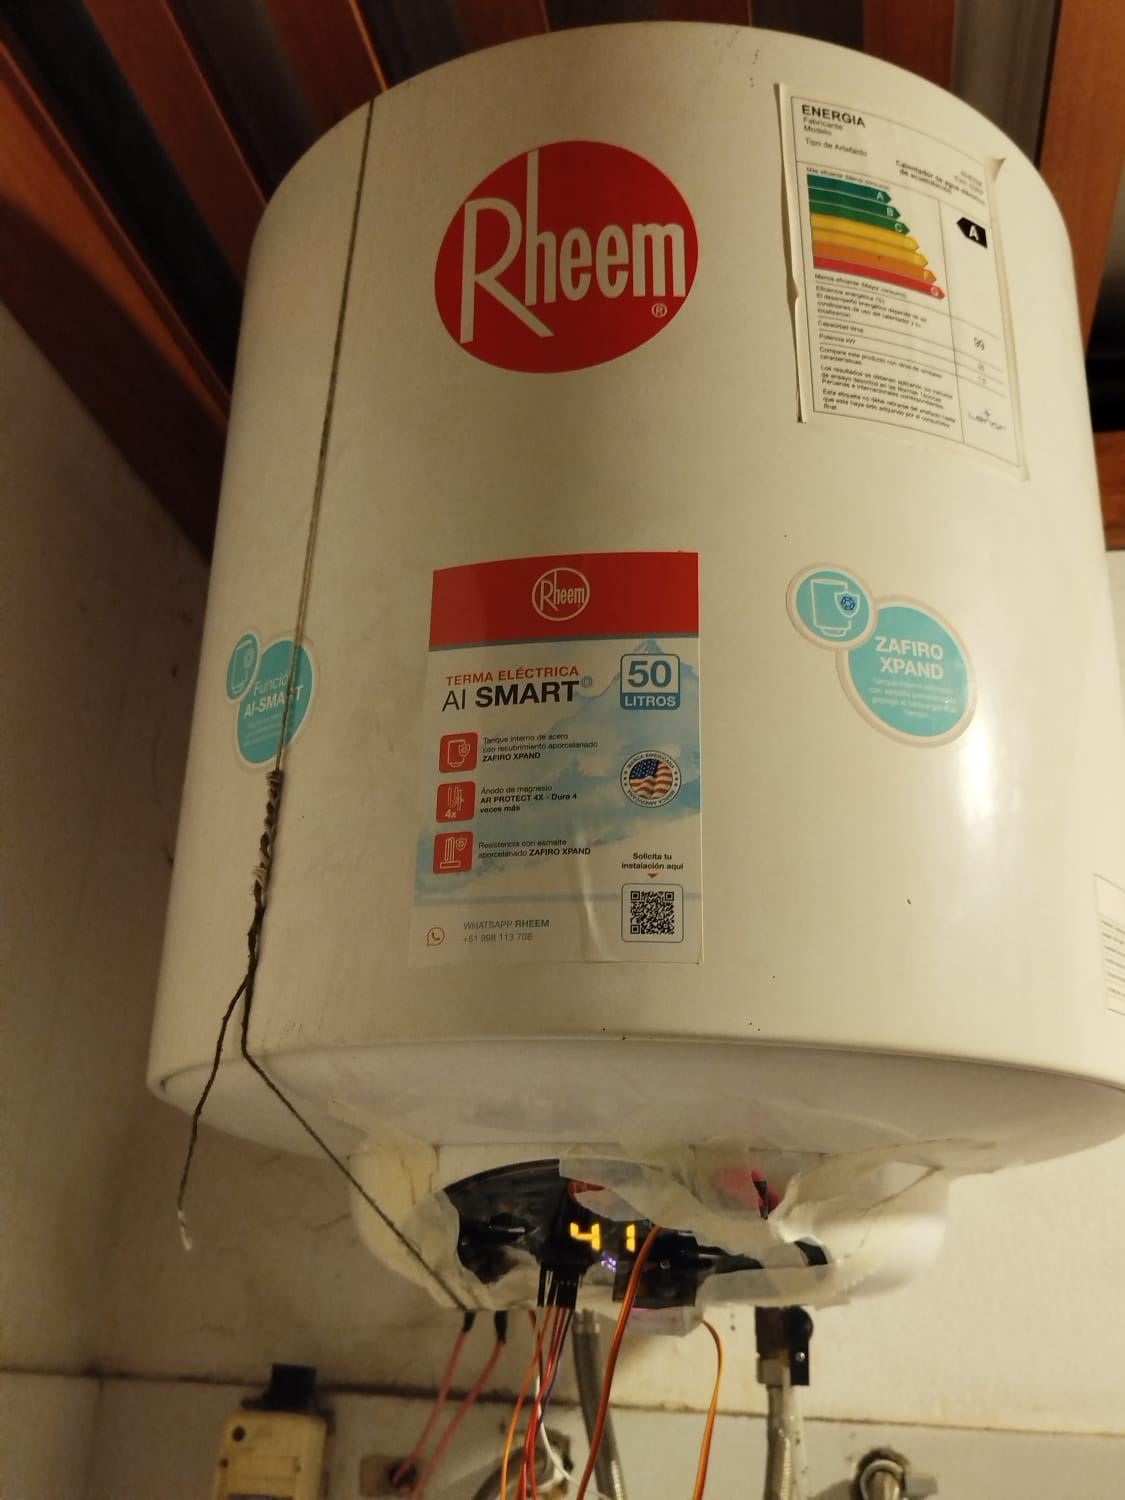
\includegraphics[height=6cm,keepaspectratio]{figures/prototype.jpg}\hspace{8mm}
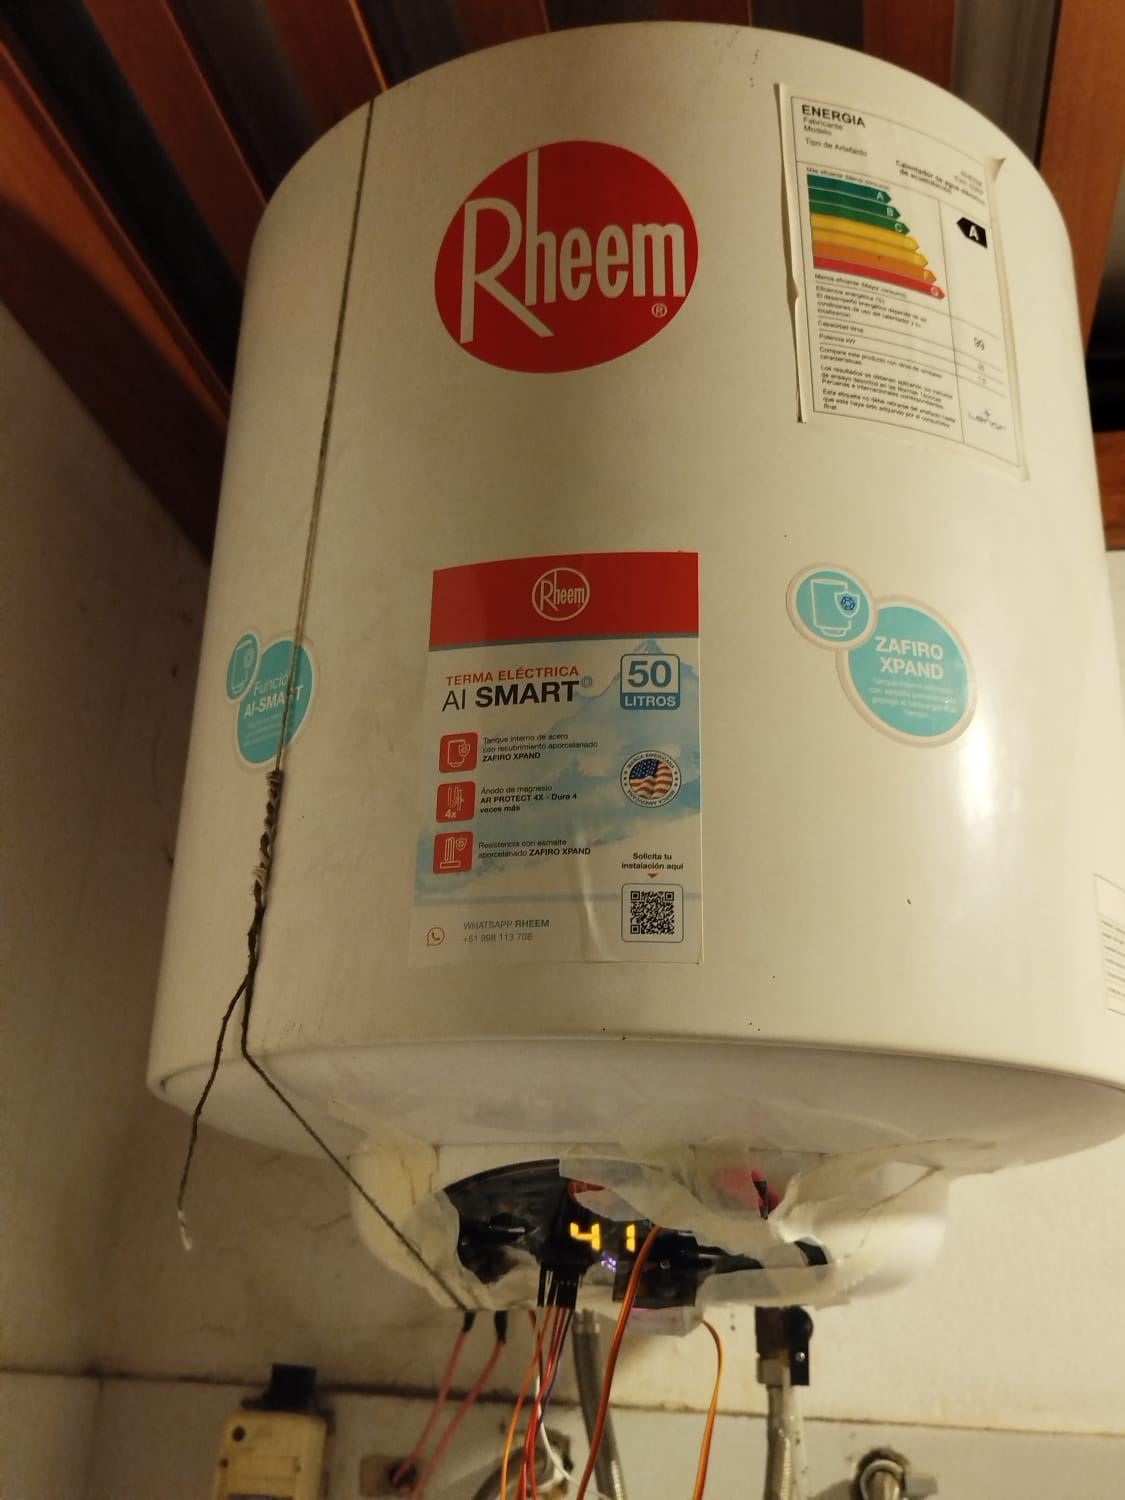
\includegraphics[width=0.5\linewidth,trim=150bp 0bp 100bp 1000bp,clip]{figures/prototype.jpg}
\caption{Tape-mounted prototype on the reference Rheem heater: overall view and detail of the panel mounting. The original visor shows 41~$^\circ$C in this photograph. The mounting provides a physical reference for optical alignment and servo travel.}
\label{fig:prototype}
\end{figure}

%% \section{Results}
%% \Needspace{6\baselineskip}
\subsection{Mounted Pilot Calibration}
Table~\ref{tab:rgb} and Figure~\ref{fig:rgb-results} summarize the raw calibration readings. The red condition has a dominant red response and substantially higher total light than the green condition. The green reference has a larger green than red component, despite much lower absolute counts. The clear channel therefore helps separate overall illumination from normalized color. The unlit condition produced small nonzero readings, making a dark threshold more appropriate than exact equality to zero.

\begin{table}[htbp]
\centering
\caption{Median raw counts transcribed from the mounted RGB calibration photographs, with 154~ms integration and 4$\times$ gain.}
\label{tab:rgb}
\begin{tabular}{lrrrr}
\toprule
Pilot condition & R & G & B & Clear \\
\midrule
Red &301&25&34&331\\
Green &17&22&8&46\\
Unlit &4&3&3&5\\
\bottomrule
\end{tabular}
\end{table}

\begin{figure}[htbp]
\centering
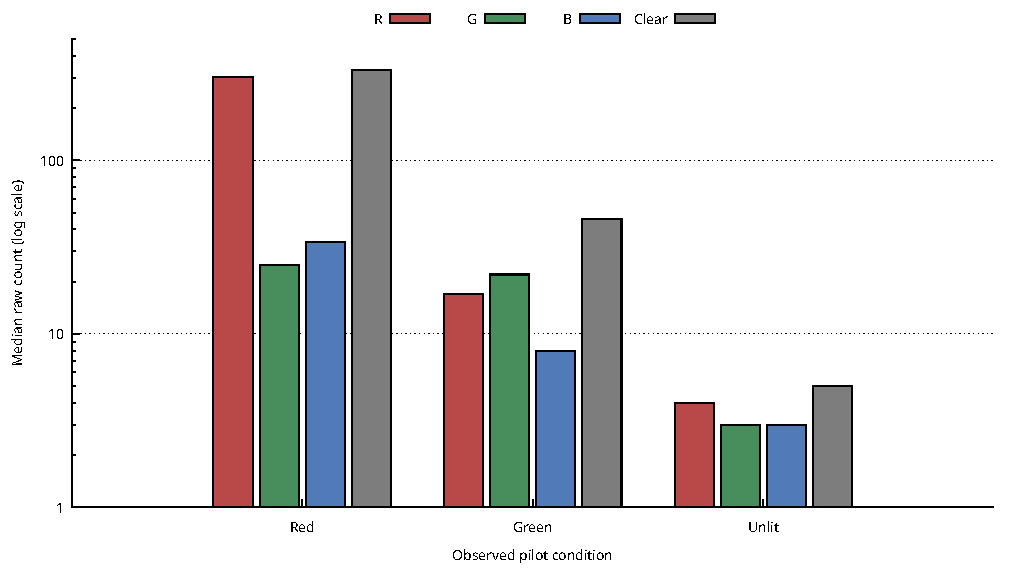
\includegraphics[width=0.88\linewidth]{figures/rgb_calibration.pdf}
\caption{Original result figure generated from the calibration readings in Table~\ref{tab:rgb}. The vertical axis is logarithmic. Each group contains the median red, green, blue, and broadband clear-channel response.}
\label{fig:rgb-results}
\end{figure}

The photographs contain overlapping readings, so the transcribed rows are not independent repetitions. These medians establish calibration references for the fixed, shielded alignment, rather than a measured classification accuracy across different lighting conditions. The selected 0.07 distance tolerance covers the recorded red and green samples; broader robustness requires testing the assembled optical geometry.

\Needspace{6\baselineskip}
\subsection{Mechanical and Software Checks}
The supervised power-button trial registered an on action with servo A configured to press at 29 degrees on the tape-mounted mechanism. Its configured rest position is 0 degrees. This is an angular setting for that mounting, not a measurement of contact force or repeated-actuation reliability. The photograph in Figure~\ref{fig:prototype} provides the corresponding appliance context.

Table~\ref{tab:control-checks} summarizes the software checks performed on the integrated implementation. The backend suite passed 20 tests, and the embedded adjustment checks exercised all 46$\times$46 pairs of allowed initial and target setpoints. Host checks used the actual heater-control header with stubbed peripherals, so these results verify command decisions separately from mechanical behavior.

\begin{table}[htbp]
\centering
\caption{Verified software behavior and its interpretation.}
\label{tab:control-checks}
\small
\begin{tabularx}{\linewidth}{@{}P{3.2cm}L@{}}
\toprule
Check & Observed result \\
\midrule
Unknown startup state & No automatic toggle is issued to discover power; unknown setpoint remains unsynchronized.\\
Standby command & Wake is separated from the requested action, which waits for a fresh pilot observation.\\
Missing confirmation & The pending action is cancelled without repeating wake presses indefinitely.\\
Circular setpoint & The 30-to-75 downward boundary and 75-to-30 upward boundary are one-step software transitions.\\
Temperature distinction & Captures taken during adjustment remain unavailable as measured water temperature until a later capture.\\
User cancellation & A later on request can cancel a pending off action during the wake sequence.\\
\bottomrule
\end{tabularx}
\end{table}

The controller firmware compiled successfully. Together with the optical and button observations, these checks support the separation of sensing, decision logic, and physical actuation. They do not quantify water-use accuracy or energy savings; the prototype reports panel observations and configured pulse-based quantities rather than independently calibrated tank temperature or electrical consumption.

\section{Market Description}
\input{market_descrp.tex}
%% \section{Conclusion}
%% The prototype combines external panel sensing, an embedded button controller, and a local wireless application around the Rheem EW1-50RP. Mounted calibration produced distinguishable red, green, and unlit RGBC responses, including small nonzero dark readings. A supervised tape-mounted power-button trial registered a press at a configured angle of 29 degrees. These results provide concrete optical and mechanical references for the assembled device.

Separating current temperature from setpoint was essential to the control logic because the panel flashes the selected value during adjustment. The implemented wake sequence likewise distinguishes standby from power-off without converting an OCR failure into an off observation. Backend, host, and embedded adjustment checks verified these decisions and the circular selection range; physical repeatability remains dependent on the final alignment and servo travel.

Calibration should be repeated after changing the optical cover or mechanical mounting, and the settling interval should be matched to the observed panel behavior. Future work can build on flow measurements to compare accumulated volume across operating periods. The application API can also support voice interaction through the same validated monitoring and control operations already used by the dashboard.

\bibliographystyle{ACM-Reference-Format}
\bibliography{references}
\end{document}
